\documentclass[a4paper,12pt]{article}

\title{Exercise 2: Obstacle Avoidance}
\author{Gruppe 6}

\usepackage[T1]{fontenc}
\usepackage[utf8]{inputenc}
\usepackage[british]{babel}
\usepackage{microtype}

\usepackage{amsmath}
\usepackage{libertine}

\usepackage{graphicx}

\usepackage[hidelinks]{hyperref}

\setlength{\parskip}{1ex}
\setlength{\parindent}{0pt}
\setlength{\parfillskip}{30pt plus 1 fil}

\begin{document}

\maketitle

\section{Measurements}

We started by measuring the robot's front IR sensor on seven distances: 0 cm, 10
cm, 20 cm, 30 cm, 40 cm, 50 cm, and 60 cm.  We positioned the robot in front of
pieces of paper in a lit room and had it make 20 IR measurements at each
distance.  The distance was from the robot's bumper to the piece of paper.


\section{Driving}

\subsection{Issue: Pull mode vs. push mode}

We had a problem with wrong IR readings on the Scorpion robots \emph{and} in the
Stage simulator.  When not constantly calling the \texttt{Read()} function, the
\texttt{libplayer} API sometimes gave us old readings instead of current ones.
After doing some research, we found out that the issue was because of how the
default data mode was used by
\texttt{libplayer}\footnote{\url{http://playerstage.sourceforge.net/doc/Player-cvs/player/group__libplayerc__datamodes.html}}.
By default it uses PULL mode.  This mode sends messages to the client when asked
to, but if the client does not read often enough, buffer overflows in the server
queue can occur.  To get rid of this problem, and not have to call
\texttt{Read()} all the time, we have set a \texttt{libplayer} replace rule:

\begin{verbatim}
robot.SetReplaceRule(true, PLAYER_MSGTYPE_DATA, -1, -1);
\end{verbatim}

This rule tells \texttt{libplayer} to ignore the buffer queue and just replace
every old measurement with every new measurement, thus ensuring that
\texttt{Read()} gets us the newest measurement.


\subsection{Abortmission}

Our first test program Abortmission worked by driving straight forward at 20 cm/sec forever. While checking every 20 ms, if the front ir sensor detected anything within 50 cm. If so we would turn 180 degrees/sec left or right for 1 secound. We determined the turning direction by comparing the distance readings of the left and right ir sensor relative to the center ir sensor, shown as red and blue in figure 1. We always turn towards the longest sensor reading of the two. If they were equal we would turn right.
\newline
\newline
This solution just barely worked, since it only used the front sensor and arbitrability just turned 1 secound in the chosen direction.

\begin{figure}
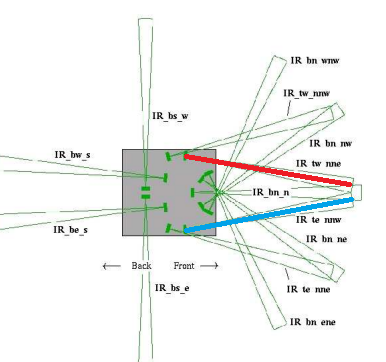
\includegraphics{robot2.png}
\caption{Robot sensors}
\end{figure}

\subsection{Sensor-validate}

We initially implemented Sensor-validate to only belive a sensor if it read out a valid distance within our threshold 10 times in a row, otherwise its counter would be reset. This was to ignore invalid readings but ended up making us never belive any sensors. Therefore we changed it to just see any sensor reading, within our threshold, as a potential collision.
\newline
\newline
Sensor-validate

Mark skriver noget?

\end{document}
